
\section{Algorithms}


\citet*{kahn:1995} gave the the first polynomial-time algorithm achieving the
bound $\BigO{\log e(\P)}$ up to a constant factor in 1995. The idea of their
algorithm is to solve a convex optimization problem to compute the entropy
\(H(\P)\). With \ref{eq:khankim1} this entropy can be used to approximate
\(e(\P)\) which can help to choose a good query. With this technique, one can
choose a good query at each step in polynomial-time. However, this algorithm
is not practical as (for the moment) it requires to use the ellipsoid
algorithm as a subroutine.

Finally, in 2013, \citet*{cardinal:2013} provide new methods. Three new
algorithms are studied. Those three algorithms all have the same canvas: a
first polynomial-time preprocessing phase followed by a $\BigO{\log e(\P)}$
query phase. Caution has to be made though: each of the three different
algorithms match the ITLB for a subset of the problem instances.

\begin{table}
	\begin{center}
	\caption{We denote by $E A(n)$ the time needed for the ellipsoid algorithm
to compute the entropy of a poset of order $n$. The original bound given by
\citet*{kahn:1995} on the number of comparisons performed by their algorithm is
$54.45 \cdot \log e(\P)$. The improved bound given in the table is a byproduct
of the results of \citet*{cardinal:2013}. The notation $\BigOe{n}$ means
that the hidden constant may depend on $\epsilon$.}
	\label{tree:supi:table/jcardin}
	\begin{tabular}{|c|c|c|}

	\hline
	Algorithm & Global Complexity & Number of comparisons\\\hline\hline
	\citet*{kahn:1995} & $\BigO{n \log n \cdot E A(n)}$ & $\leq 9.82 \cdot \log
e(\P)$\\\hline\hline
	\citet*{cardinal:2013} \textbf{1} & $ \BigO{n^{2}} $ & $\BigO{\log n \cdot
\log e(\P)}$ \\\hline
	\citet*{cardinal:2013} \textbf{2} & $ \BigO{n^{2.5}} $ & $\leq (1 +
\epsilon) \log e(\P) + \BigOe{n}$ \\\hline
	\citet*{cardinal:2013} \textbf{3} & $ \BigO{n^{2.5}} $ & $\leq 15.09 \cdot
\log e(\P)$ \\\hline

	\end{tabular}
	\end{center}
\end{table}


\ref{tree:supi:table/jcardin} highlights the properties of the different
algorithms, \ie:

\begin{itemize}

\item If $\log e(\P)$ is super-linear in $n$, the number of comparisons of
\citet*{cardinal:2013} \textbf{2} is lower than that of \citet*{kahn:1995}. By
optimizing over $\epsilon$, it can be shown that the number of comparisons is
actually $\log e(\P) + \SmallO{\log e(\P)} + \BigO{n}$ in this case, a number of
comparisons comparable to that of Fredman’s algorithm;

\item If $\log e(\P)$ is linear or sub-linear in $n$, the number of comparisons
of \citet*{cardinal:2013} \textbf{3} is comparable to that of
\citet*{kahn:1995}, although the constant in front of $\log e(\P)$ is still far
from the best constant achieved by a super-polynomial algorithm via balancing
pairs (see \citet*{brightwell1995balancing} and
\citet*{brightwell1999balanced});

\item Algorithms from \citet*{cardinal:2013} have the following useful
property: they compute information that guides the sorting and can then be
reused to solve any given instance with the same partial information $\P$, in
time proportional to the number of comparisons, plus a term linear in $n$.

\end{itemize}

The idea of \citet*{cardinal:2013} is to remove some information from the input
poset to produce a weak subposet \(\P'\) (whose refinement is \(\P\)) for which
computing a linear extension is \BigO{\log e(\P')} and whose entropy is not to
far from the entropy of the original poset. Since \(H(\P)\) is
\BigTheta{e(\P)}, as it was proved by \citet*{kahn:1995}, one can analyze what
``not to far'' means for a given information removal technique.

For example, one can iteratively extract a maximal chain of the input poset
computing a so-called greedy chain decomposition. Once this is done, we
erase all the relations of the input existing between elements of two different
chains of the decomposition. One can then merge the chains using the optimal
Huffman Merging algorithm we described in \ref{tree:merging:kgeq3}.
\ref{fig:supi/alg2} illustrates this technique and is in fact a description of
algorithm \textbf{2} of \citet{cardinal:2013}. The two other algorithms of
\citet*{cardinal:2013} are variants of this approach.

The same idea was already present in \citet*{cardinal:2010}. Then, the problem
to solve was Partial Order Production which is the complementary problem to
Sorting under Partial Information. In this case, we look at antichains rather
than chains of the input poset and instead of removing known information we ask
the algorithm to compute more information than required. The relation between
those problems is explained in detail in \cite{DBLP:conf/birthday/CardinalF13}.

\begin{figure}
	\centering
	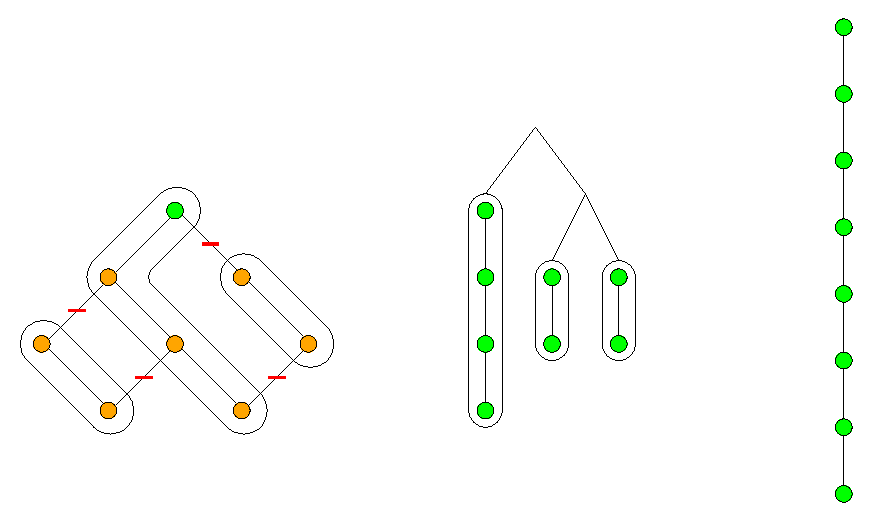
\includegraphics[height=0.2\textheight]{fig/supi/reduction:diag}
	\caption{\label{fig:supi/alg2} Illustration of the second algorithm in
\citet*{cardinal:2013}.}
\end{figure}


Note that randomized algorithms also exist for this purpose. The idea is to
evaluate the quality of a comparison by generating a sample of possible linear
extensions, count the number of times the answer to this question \(x
\ask{\le} y\) is true and then only ask the question if the ratio of
this count over the total number of sampled linear extensions lies within a
fixed interval $[q, 1-q], 0 < q \le \frac{1}{3}$. See \citet*{huber2006fast} for
more.

